\documentclass{article}


\usepackage{fontspec}
\defaultfontfeatures{Scale=MatchLowercase,Mapping=tex-text}
\setmainfont[Ligatures=TeX]{DejaVu Serif}
\setsansfont[Ligatures=TeX]{DejaVu Sans}
\setmonofont{DejaVu Sans Mono}

\usepackage{hyperref} % For hyperlinks in the PDF
\usepackage{adjustbox} % For resizing
\usepackage{graphicx} % For spaces in pictures
\usepackage[space]{grffile} % Same
\usepackage[margin=0.5in]{geometry} % Adjust margins

\usepackage{fancyvrb}
\newenvironment{myverb}{% Verbatim shrinked
 \VerbatimEnvironment
 \begin{adjustbox}{max width=\linewidth}
 \begin{BVerbatim}
  }{
  \end{BVerbatim}
 \end{adjustbox}
}

%----------------------------------------------------------------------------------------
%	TITLE SECTION
%----------------------------------------------------------------------------------------

\title{\vspace{-15mm}\fontsize{24pt}{10pt}\selectfont\textbf{ChIP-Seq peaks classification}} % Article title

\author{
\large
\textsc{Oleg Shpynov}\\
\normalsize \href{mailto:oleg.shpynov@jetbrains.com}{oleg.shpynov@jetbrains.com} % Your email address
\vspace{-1mm}
}
\date{\today}

%----------------------------------------------------------------------------------------

\begin{document}

\maketitle % Insert title
\tableofcontents % Print the contents section

%----------------------------------------------------------------------------------------
%	ARTICLE CONTENTS
%----------------------------------------------------------------------------------------

\section{Introduction}
The goal of this work is to answer the question:
\textit{How to distinguish narrow and broad ChIP-Seq peaks?}
ENCODE project standards\\
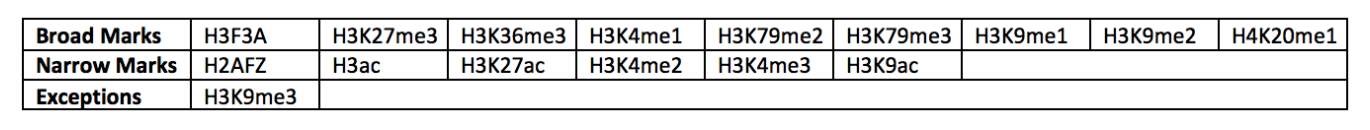
\includegraphics[width=\linewidth]{encodestandards.png}\footnote{\url{https://www.encodeproject.org/data-standards/chip-seq/}}

\section{Methods and tools}
We used ENCODE dataset GSE26320 to estimate ChIP-Seq peak length distribution. It is was shown that different ChIP-Seq modification has different biological function and demonstrate different patterns across genome. \textbf{TODO}\\
In order to deal with epigenomic data in human readable predicate way it is quite natural to have the ability to classify ChIP-Seq peaks by distribution, shape, intensity, length, etc.\\
To address this question we performed a simple experiment, which allowed us to compare peaks characteristics provided by different peak callers. We've used gold-standard peak callers: MACS2, SICER as well peak caller ZINBRA.\\

\subsection{Experiment design}
\begin{itemize}
\item Download GSE26320 dataset
\item Align all reads to hg18 using bowtie with default params
\item Launch MACS2, SICER and ZINBRA to produce peaks
\item Aggregate peaks, produced for different ChIP-Seq tracks by distinct histone modifications
\item Filter out outliers by processing only 10-90 percentile of all values
\item Analyze peaks length distribution for different histone modifications 
\item Formulate criterion to classify peaks into narrow and broad classes
\end{itemize}
For each tool we plot aggregated peak lengths distribution and boxplots for each histone mark.
\section{SICER}
SICER is a tool, which supports peak calling for both narrow and broad peaks out of the box, so that we used it as reference.
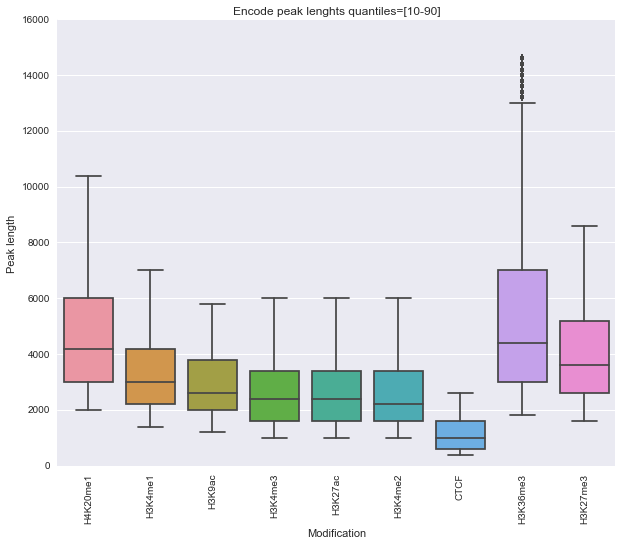
\includegraphics[width=0.5\linewidth]{sicer.png}
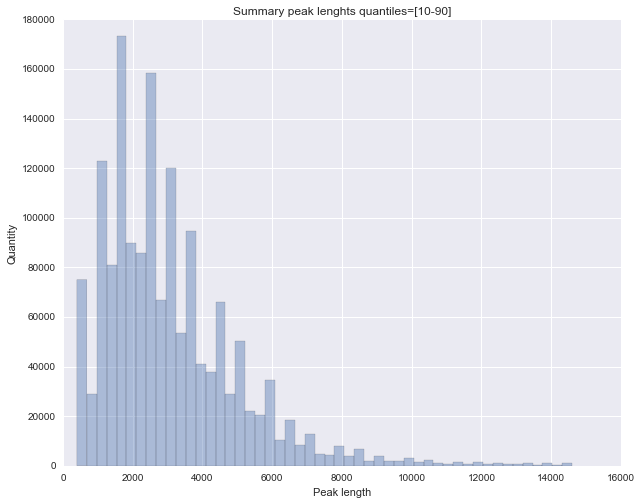
\includegraphics[width=0.5\linewidth]{sicer2.png}

\section{ZINBRA}
ZINBRA uses single statistical model for both narrow and broad peaks, producing enrichment states for binned(default bin size = 200, which corresponds to typical nucleosome size) genome, concatenating adjacent enriched bins into wider peaks.
\subsection{FDR = 0.0001}
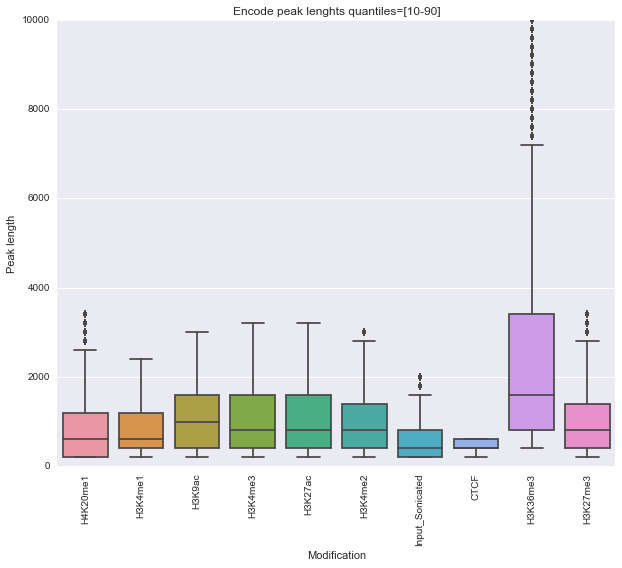
\includegraphics[width=0.5\linewidth]{zinbra.png}
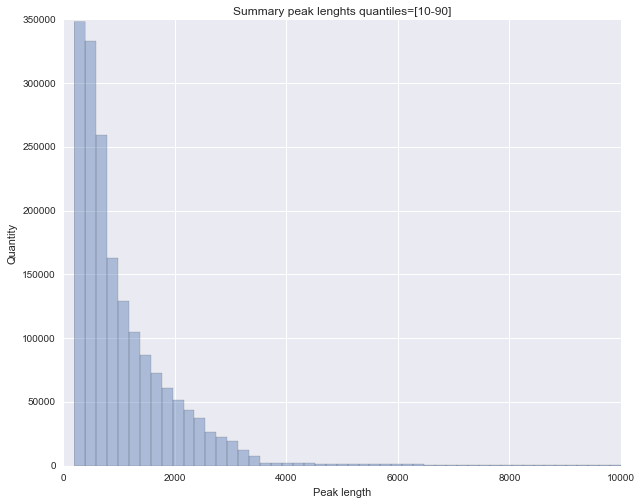
\includegraphics[width=0.5\linewidth]{zinbra2.png}

\subsection{FDR = 0.001}
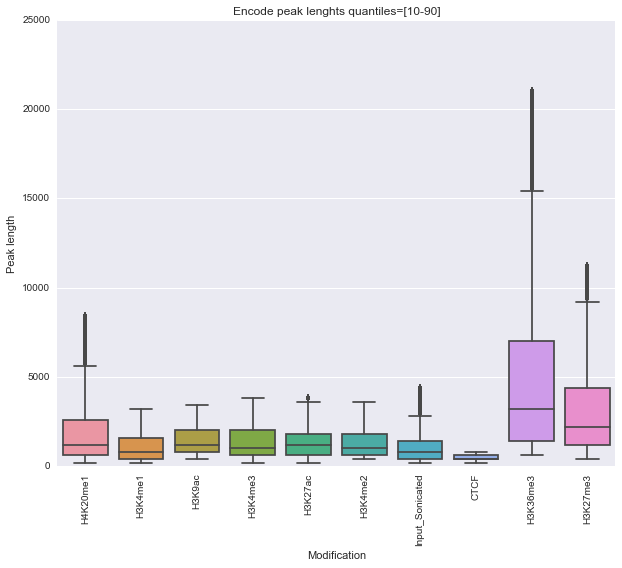
\includegraphics[width=0.5\linewidth]{zinbra1e3.png}
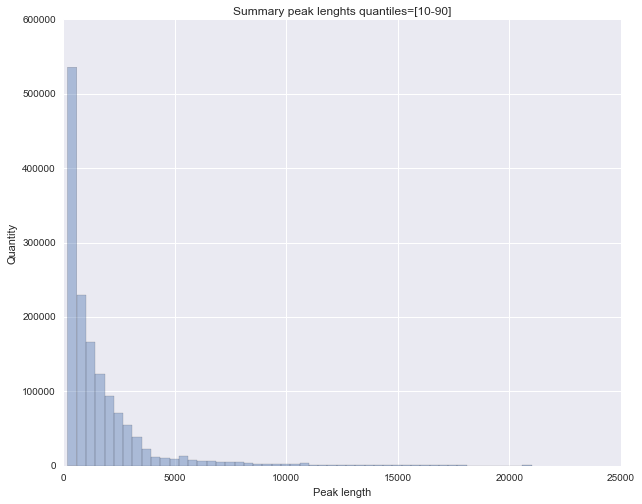
\includegraphics[width=0.5\linewidth]{zinbra1e32.png}

\subsection{FDR = 0.01}
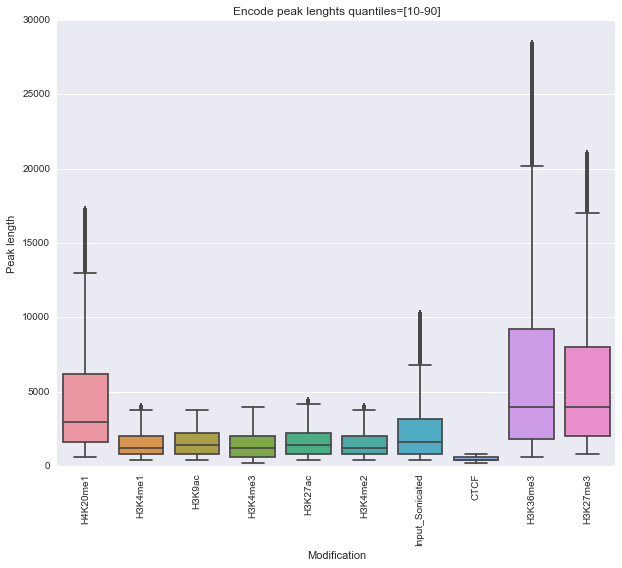
\includegraphics[width=0.5\linewidth]{zinbra1e2.png}
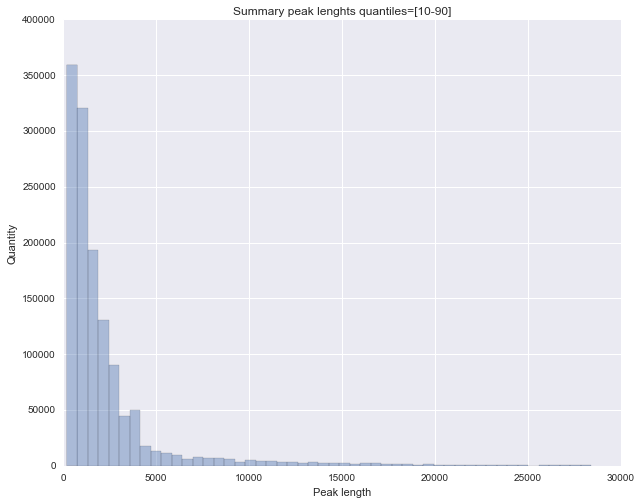
\includegraphics[width=0.5\linewidth]{zinbra1e22.png}

\section{ZINBRA with extended peaks}
Motivation: in ChIP-Seq enrichment predicates, decision on whether given locus is enriched or not is made according to the fraction of enriched bins within. So that we decided to extend enriched regions (adjacent enriched bins) in following manner: extend each region as much as possible, so that fraction of enriched bins is $\geq$ threshold $k=0.5$. 
\subsection{Extended peaks FDR = 0.0001 K = 0.5}
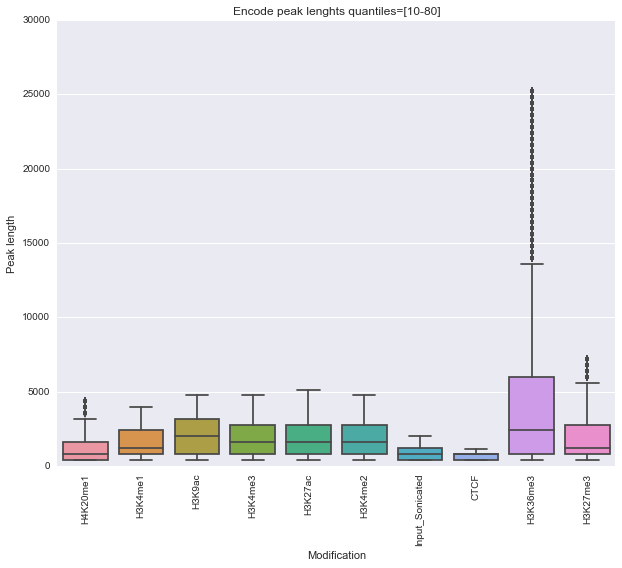
\includegraphics[width=0.5\linewidth]{zinbra0.5.png}
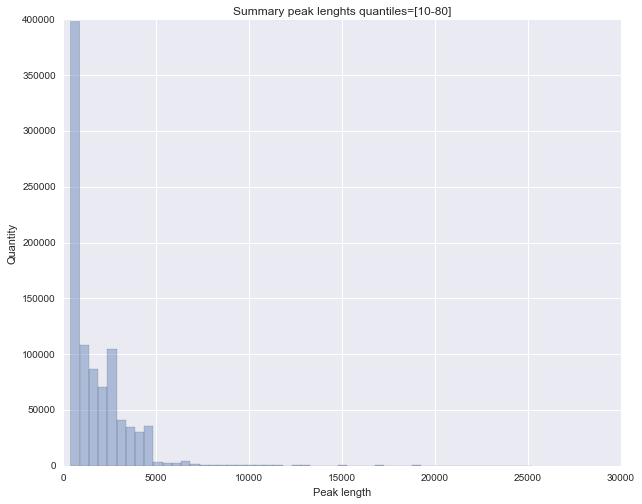
\includegraphics[width=0.5\linewidth]{zinbra0.52.png}

\subsection{Extended peaks FDR = 0.001 K = 0.5}
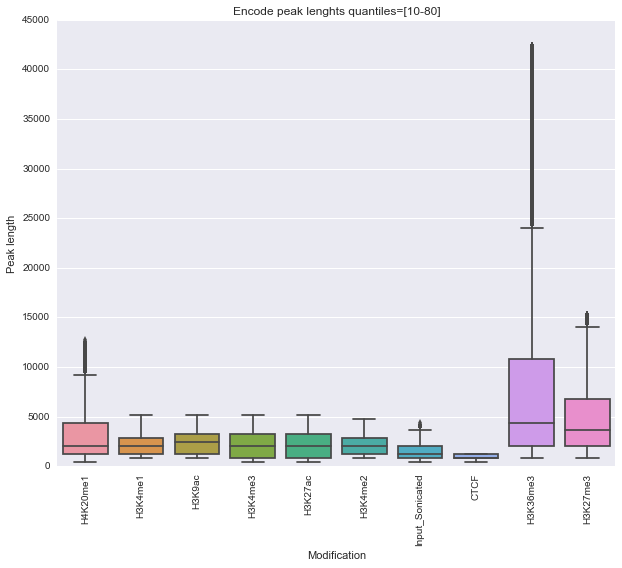
\includegraphics[width=0.5\linewidth]{zinbra1e30.5.png}
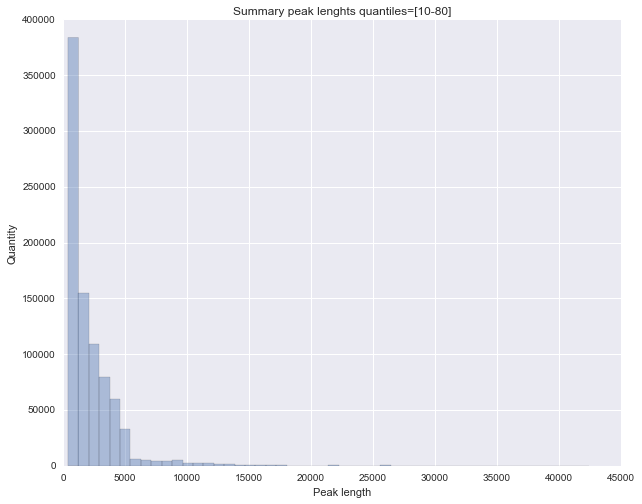
\includegraphics[width=0.5\linewidth]{zinbra1e30.52.png}

\section{MACS2}
MACS2 by default deals with narrow peaks, however it has \textit{--broad} command line options to process broad peaks as well.
\subsection{MACS2 Broad}
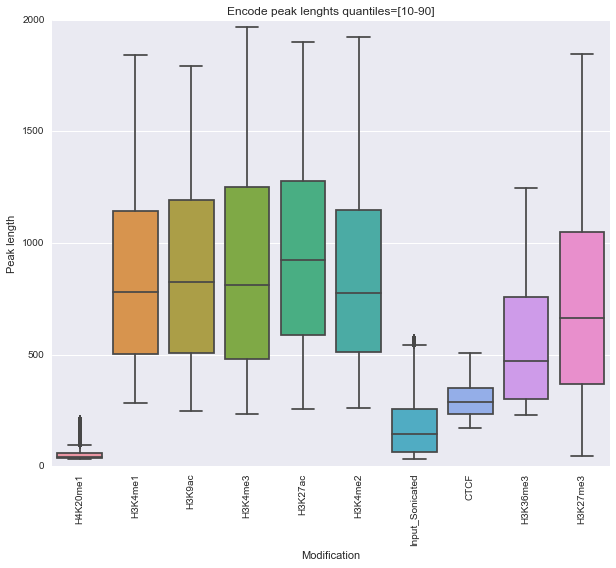
\includegraphics[width=0.5\linewidth]{macs2broad.png}
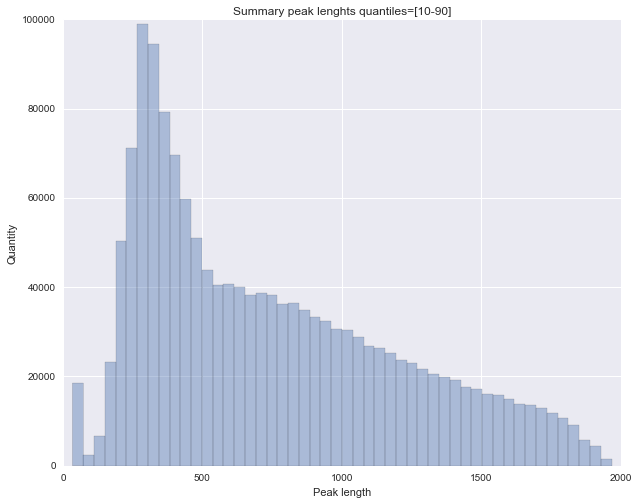
\includegraphics[width=0.5\linewidth]{macs2broad2.png}

\subsection{MACS2 Narrow}
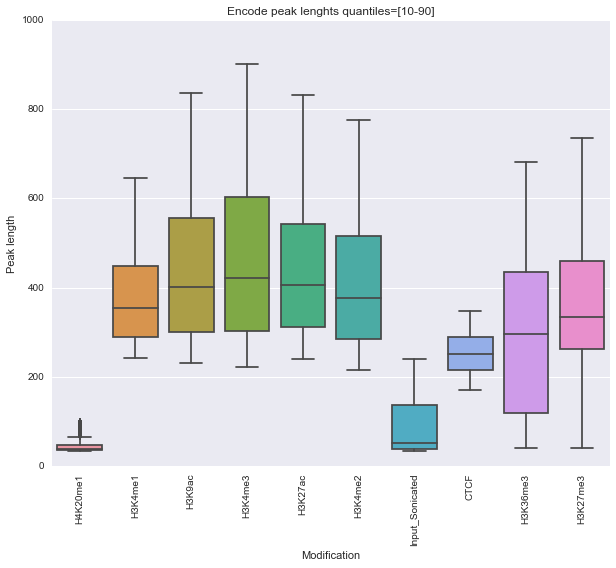
\includegraphics[width=0.5\linewidth]{macs2.png}
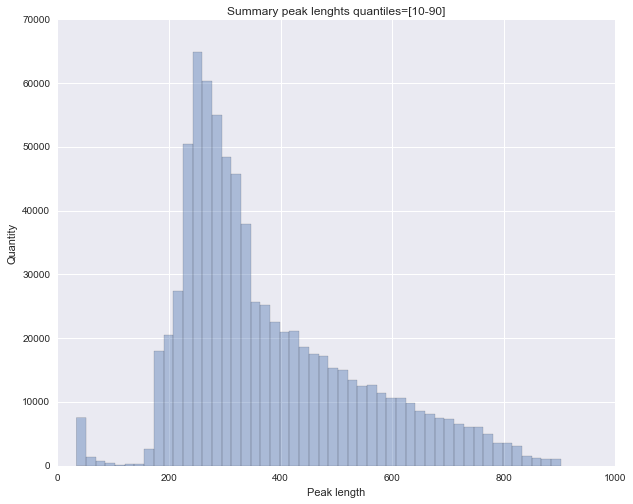
\includegraphics[width=0.5\linewidth]{macs22.png}

\subsection{MACS2 Narrow with control}
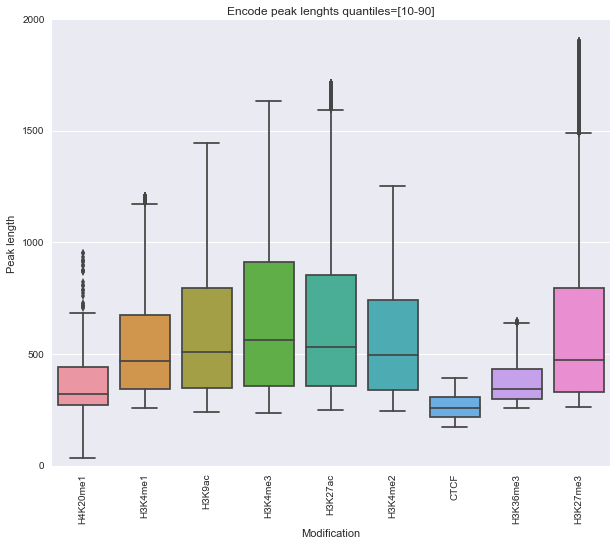
\includegraphics[width=0.5\linewidth]{macs2control.png}
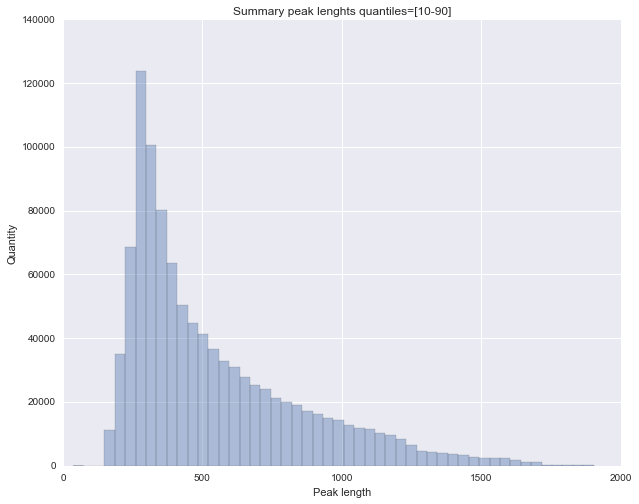
\includegraphics[width=0.5\linewidth]{macs2control2.png}

\section{ENCODE}
Automatic processed hg19 encode project peaks.\\
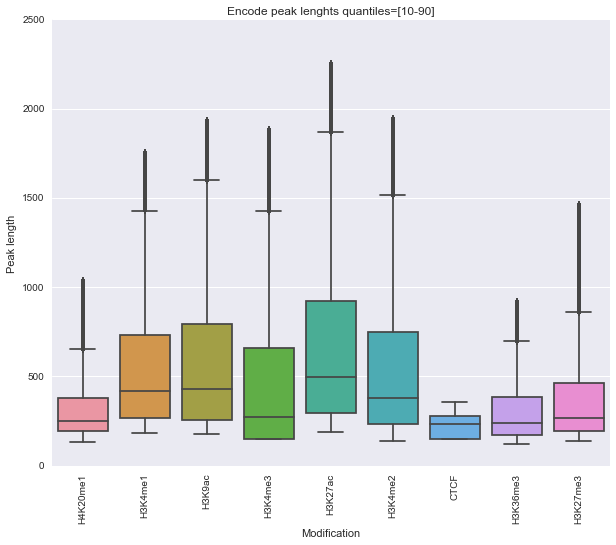
\includegraphics[width=0.5\linewidth]{encodepeaks.png}
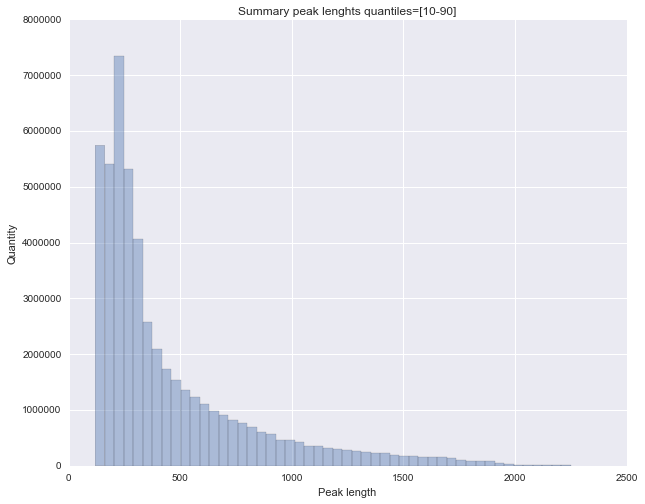
\includegraphics[width=0.5\linewidth]{encodepeaks2.png}

\section{Discussion}
The evidence shows that MACS2 can hardly be used to estimate both narrow and broad peaks. Even MACS2 in \textit{--broad} mode fails to classify H3K36me3 as broad peaks, since it is known to be associated with gene body.\\
Comparing SICER and ZINBRA seems tricky, since FDR correction plays crucial role in peak length distribution. \\
ZINBRA with $fdr=10^{-3}$ results in the closest distribution to SICER. Moreover we can see, that peak extension doesn't make sense for $fdr=10^{-3}$.\\ Also threshold 3kbp looks natural to separate narrow and broad peaks.\\

Conclusion:
\begin{itemize}
\item ZINBRA is in general consistent with MACS2 in terms of narrow peaks, and with SICER in terms of broad peaks.
\item SICER and ZINBRA are most consistent in terms of peaks distribution for ZINBRA $fdr=10^{-3}$.
\item MACS2 is not capable to call broad peaks even with \textit{--broad} command line option.
\item {Q: \textit{How to distinguish narrow and broad ChIP-Seq peaks?}\\
A: Peak can be considered as \textit{broad} if length is at least 3kbp.
}
\end{itemize} 

\end{document}
